\documentclass[12pt, a4paper]{article}
\usepackage[utf8]{inputenc}
\usepackage[spanish]{babel}
\usepackage{amsmath}
\usepackage{graphicx}
\usepackage{listings}
\usepackage{xcolor}
\usepackage{float}
\usepackage[margin=2.54cm]{geometry}
\usepackage{listingsutf8}
\usepackage{graphicx}

% Configuración para código R
\lstset{
    inputencoding=utf8,               % Para soportar UTF-8
    extendedchars=true,               % Manejo de caracteres extendidos
    language=R,                       % Lenguaje del código
    basicstyle=\ttfamily\small,       % Estilo básico de texto
    keywordstyle=\color{blue},        % Color de palabras clave
    stringstyle=\color{red},          % Color para strings
    commentstyle=\color{green!60!black}, % Color para comentarios
    numbers=left,                     % Numeración a la izquierda
    numberstyle=\tiny,                % Estilo de los números
    numbersep=5pt,                    % Separación de los números
    backgroundcolor=\color{gray!10},  % Color de fondo
    frame=single,                     % Marco alrededor del código
    breaklines=true,                  % Romper líneas largas
    breakatwhitespace=true,           % Romper en espacios en blanco
    showstringspaces=false            % No mostrar espacios en strings
}


\title{Informe de Examen de Estadística y Probabilidad}
\author{Universidad Nacional Hermilio Valdizán\\Facultad de Economía}
\date{\today}

\begin{document}

\maketitle

\textbf{Estudiante: Palomino Ricaldi Antony}

\section{Problema 1: Derivación de la Fórmula de la Moda para Datos Clasificados}

La fórmula de la moda para datos clasificados se expresa como:

\[Mo = L_i + A \cdot \left(\frac{f_i - f_{i-1}}{(f_i - f_{i-1}) + (f_i - f_{i+1})}\right)\]

Donde:
\begin{itemize}
    \item $L_i$ = Límite inferior de la clase modal
    \item $A$ = Amplitud del intervalo
    \item $f_i$ = Frecuencia de la clase modal
    \item $f_{i-1}$ = Frecuencia de la clase anterior a la modal
    \item $f_{i+1}$ = Frecuencia de la clase posterior a la modal
\end{itemize}

\section{Problema 2: Análisis de Ventas de Gasolina}

\subsection{Planteamiento del Problema}
Se analizan las ventas de gasolina de una refinería de Petro-Perú en Ica, con datos clasificados en intervalos de 10,000 galones.

\subsection{Solución en R}

\begin{lstlisting}[caption=Análisis de Ventas de Gasolina]

# Crear el dataframe con los datos
ventas_gasolina <- data.frame(
    intervalo_inferior = seq(0, 70, by = 10),
    intervalo_superior = seq(10, 80, by = 10),
    frecuencia = c(10, 20, 30, 25, 15, 10, 5, 5)
)

# Calcular marca de clase
ventas_gasolina$marca_clase <- (
    ventas_gasolina$intervalo_inferior +
    ventas_gasolina$intervalo_superior
) / 2

# a) Calculo del total de galones vendidos
total_galones <- sum(
    ventas_gasolina$marca_clase *
    ventas_gasolina$frecuencia
)

# b) Media de galones por operacion
n_operaciones <- sum(ventas_gasolina$frecuencia)

media_galones <- total_galones / n_operaciones

# c) Moda
clase_modal <- which.max(ventas_gasolina$frecuencia)
Li <- ventas_gasolina$intervalo_inferior[clase_modal]
A <- 10 # Amplitud del intervalo
fi <- ventas_gasolina$frecuencia[clase_modal]
fi_anterior <- ventas_gasolina$frecuencia[clase_modal - 1]
fi_posterior <- ventas_gasolina$frecuencia[clase_modal + 1]

moda <- Li + A * (
    (fi - fi_anterior) / ((fi - fi_anterior) + (fi - fi_posterior))
)

# d) Calcule la mediana de las ventas.
ventas_gasolina$f_a_acumulada <- cumsum(ventas_gasolina$frecuencia)

intervalo_medinal <- which(
    ventas_gasolina$f_a_acumulada >= n_operaciones / 2
)[1]

Li <- ventas_gasolina$intervalo_inferior[intervalo_medinal]
fi <- ventas_gasolina$frecuencia[intervalo_medinal]
Fi_1 <- ventas_gasolina$f_a_acumulada[intervalo_medinal - 1]

mediana <- Li + A / fi * (n_operaciones / 2 - Fi_1)    

\end{lstlisting}

\subsection{Resultados e Interpretación}

\begin{enumerate}
    \item \textbf{Total de galones vendidos}: 3 900 (miles)
    \begin{itemize}
        \item \textit{Interpretación}: La refinería vendió aproximadamente 3 900 000 galones de gasolina durante la semana.
    \end{itemize}
    
    \item \textbf{Media de galones por operación}: 32.5 (miles)
    \begin{itemize}
        \item \textit{Interpretación}: En promedio, cada operación de venta fue de aproximadamente 32 500 galones.
    \end{itemize}
    
    \item \textbf{Moda}: 26.66667 (miles)
    \begin{itemize}
        \item \textit{Interpretación}: El volumen de venta más frecuente se encuentra en aproximadamente 26 667 galones, lo cual está por encima de 25 000.
    \end{itemize}
    \item \textbf{Mediana de las ventas:} 30 (miles)
    \begin{itemize}
        \item \textit{Interpretación}: La mediana de las ventas es 30 000.
    \end{itemize}
\end{enumerate}

\section{Problema 3: Análisis de Trabajadores en Empresas}

\subsection{Solución en R}

\begin{lstlisting}[caption=Análisis de Trabajadores en Empresas]
# Obtener el valor de las variables
calculate_sturges_params <- function(data) {
    R <- diff(range(data))
    K <- ceiling(1 + 3.322 * log10(length(data)))
    A <- ceiling(R / K)

    list(
    range = range(data),
    num_classes = K,
    class_width = A
    )
}

create_frequency_table <- function(data) {
    n <- length(data)
    params <- calculate_sturges_params(data)

    # Crear le secuencia de limites
    rule <- seq(params$range[1],
    params$range[2] + params$class_width,
    by = params$class_width
    )

    # Calular el ancho de clase
    marca_de_clase <- (rule[-length(rule)] + rule[-1]) / 2

    # Crear los intervalos
    i <- cut(data, breaks = rule, right = FALSE)
    tabla <- table(i)

    # Calcular las frecuencias
    f_absoluta <- as.numeric(tabla)
    f_a_acumulada <- cumsum(f_absoluta)
    f_relativa <- f_absoluta / n
    f_r_acumulada <- cumsum(f_relativa)
    f_porcentual <- f_relativa * 100
    f_p_acumulada <- cumsum(f_porcentual)

    # Create data frame
    data.frame(
    intervalos = levels(i),
    f_absoluta = f_absoluta,
    f_a_acumulada = f_a_acumulada,
    f_relativa = f_relativa,
    f_r_acumulada = f_r_acumulada,
    f_porcentual = f_porcentual,
    f_p_acumulada = f_p_acumulada,
    marca_de_clase = marca_de_clase
    )
}

calculate_grouped_statistics <- function(freq_table, data, class_width) {
    n <- length(data)

    # Media para datos agrupados
    media_agrupada <- sum(freq_table$marca_de_clase * freq_table$f_absoluta) / n

    # Moda para datos agrupados
    intervalo_modal <- which.max(freq_table$f_absoluta)
    Li <- as.numeric(
    sub("\\[(.+),.*", "\\1", freq_table$intervalos[intervalo_modal])
    )
    fi <- freq_table$f_absoluta[intervalo_modal]
    fi_menos_1 <- if (intervalo_modal > 1) {
    freq_table$f_absoluta[intervalo_modal - 1]
    } else {
    0
    }
    fi_mas_1 <- if (intervalo_modal < nrow(freq_table)) {
    freq_table$f_absoluta[intervalo_modal + 1]
    } else {
    0
    }
    moda_agrupada <- Li + class_width *
    ((fi - fi_menos_1) / ((fi - fi_menos_1) + (fi - fi_mas_1)))

    # Mediana para datos agrupados
    intervalo_medinal <- which(freq_table$f_a_acumulada >= n / 2)[1]
    Li <- as.numeric(
    sub("\\[(.+),.*", "\\1", freq_table$intervalos[intervalo_medinal])
    )
    fi <- freq_table$f_absoluta[intervalo_medinal]
    Fi_1 <- if (intervalo_medinal > 1) {
    freq_table$f_a_acumulada[intervalo_medinal - 1]
    } else {
    0
    }
    mediana_agrupada <- Li + class_width / fi * (n / 2 - Fi_1)

    list(
    media = media_agrupada,
    mediana = mediana_agrupada,
    moda = moda_agrupada
    )
}

plot_frequency_diagram <- function(freq_table, class_width) {
    # Extraer los intervalos inferiores
    lower_bounds <- as.numeric(sub("\\[(.+),.*", "\\1", freq_table$intervalos))

    # Crear diagrama
    plot(lower_bounds, freq_table$f_a_acumulada,
    type = "s",
    xlab = "Numero de trabajadores",
    ylab = "Frecuencia acumulada",
    main = "Diagrama Escalonado con Ojiva",
    col = "blue",
    lwd = 2
    )

    # Agregar ogiva
    lines(freq_table$marca_de_clase,
    freq_table$f_a_acumulada,
    type = "b",
    col = "red",
    pch = 16,
    lwd = 2
    )

    # Agregar etiquetas
    text(freq_table$marca_de_clase,
    freq_table$f_a_acumulada,
    labels = freq_table$f_a_acumulada,
    pos = 3,
    col = "black"
    )
}

# Funcion principal para el analisis de datos
analyze_data <- function(data) {
    # Obtener las variables
    params <- calculate_sturges_params(data)

    # Crear la tabla de frecuencia
    freq_table <- create_frequency_table(data)

    # Calcular los estadisticos para datos no agrupados
    ungrouped_stats <- list(
    media = mean(data),
    mediana = median(data),
    moda = as.numeric(names(sort(table(data), decreasing = TRUE)[1]))
    )

    # Calcular los estadisticos para datos  agrupados
    grouped_stats <- calculate_grouped_statistics(
    freq_table, data, params$class_width
    )

    # Retornar los resultados
    list(
    frequency_table = freq_table,
    ungrouped_statistics = ungrouped_stats,
    grouped_statistics = grouped_stats,
    plot = function() {
        plot_frequency_diagram(freq_table, params$class_width)
    }
  )
}
\end{lstlisting}

\subsection{Fórmulas Utilizadas}

\begin{enumerate}
    \item \textbf{Media Aritmética}:
    \[ \bar{x} = \frac{\sum_{i=1}^{k} x_i \cdot f_i}{n} \]
    
    \item \textbf{Mediana para datos agrupados}:
    \[ Me = L_i + A \cdot \left(\frac{\frac{n}{2} - F_{i-1}}{f_i}\right) \]
    
    \item \textbf{Moda para datos agrupados}:
    \[Mo = L_i + A \cdot \left(\frac{f_i - f_{i-1}}{(f_i - f_{i-1}) + (f_i - f_{i+1})}\right)\]

    \item \textbf{Regla de Sturges}:
    \[ K = 1 + 3.322 \log_{10}(n) \]
\end{enumerate}

\begin{lstlisting}[caption=Numero de trabajadores encuestados por empresa]

datos_empresas <- c(
    73, 95, 61, 46, 70, 55, 87, 65,
    75, 48, 69, 75, 75, 39, 63, 82,
    58, 43, 38, 64, 69, 79, 47, 63,
    63, 81, 59, 77, 84, 34, 75, 93,
    67, 89, 66, 52, 59, 36, 62, 43,
    75, 52, 59, 87, 74, 30, 95, 38,
    50, 72, 44, 53, 68, 72, 82, 63
)

# Instancia de las funcion principal
results <- analyze_data(datos_empresas)
\end{lstlisting}

\textbf{a) Elaborar la tabla de frecuencias usando la regla de Sturges.} (2 puntos)

\begin{lstlisting}[caption=Mostrar tabla de frecuencia]
print(results$frequency_table)
\end{lstlisting}

\begin{figure}[ht!]  % El entorno figure
    \centering
    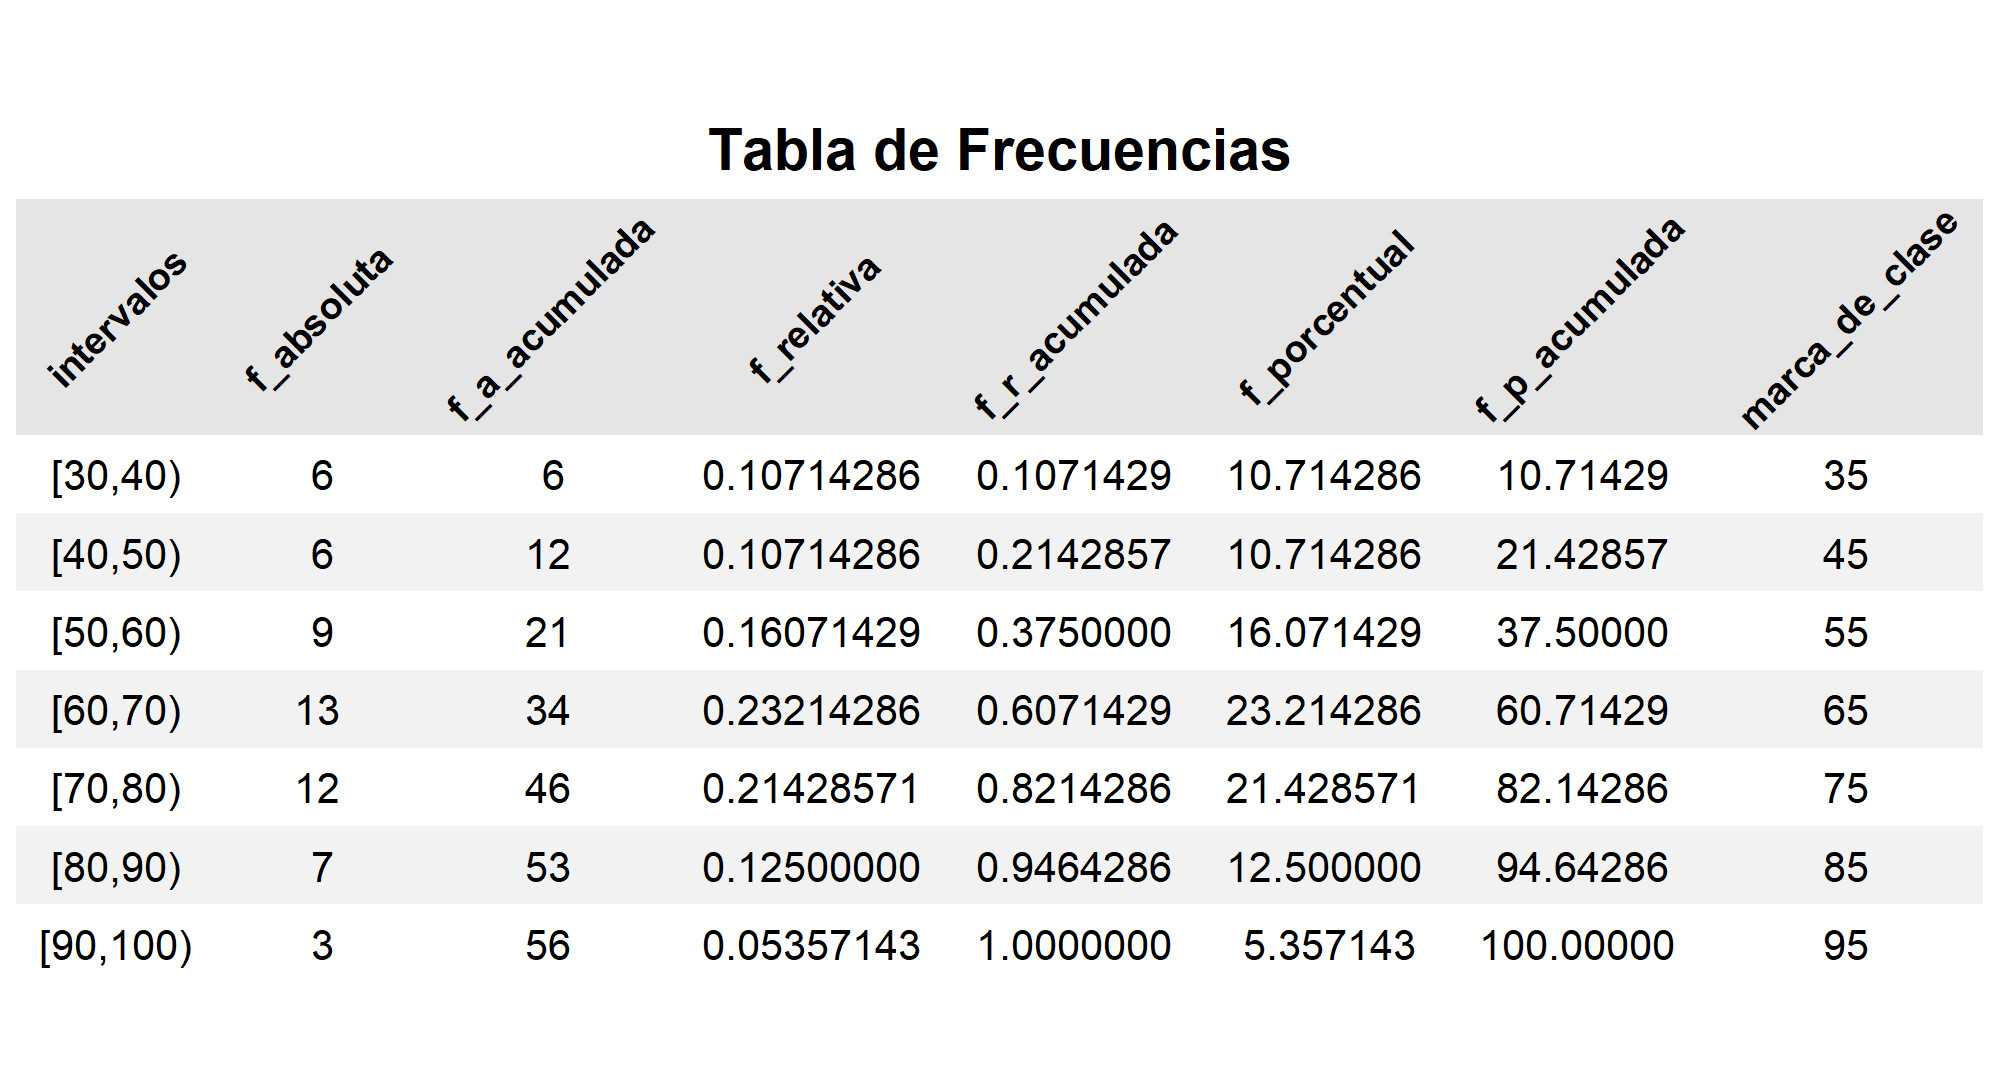
\includegraphics[width=1\textwidth]{Tabla de Distribucion de frecuencia.png}  % Ajusta el tamaño de la imagen
    \caption{Tabla de distribución de frecuencia}  % Título de la imagen
    \label{fig:ejemplo}  % Etiqueta para referenciar la imagen
\end{figure}

\textbf{b) Interpretar: $f_5$, $h_2$.} (2 puntos)

\begin{lstlisting}[caption=Obtener celdas especificas]
cat("f5:", results$frequency_table$f_absoluta[5], "\n")

> f5: 12

\end{lstlisting}

Representa la \textbf{frecuencia absoluta} del quinto intervalo, que corresponde al intervalo [70 - 80). Esto significa que hay 12 empresas cuyos encustados se encuentran dentro de este intervalo específico.

\begin{lstlisting}[caption=Obtener celdas especificas]
cat("h2:", results$frequency_table$f_relativa[2], "\n")

> h2: 0.1071429 
\end{lstlisting}

Representa la \textbf{frecuencia relativa} del segundo intervalo, que corresponde al intervalo [40 - 50). El valor 0.107 significa que la proporción de las empresas que tiene un promedio de [40 - 50) empleados encustados.

\textbf{c) Elaborar el diagrama escalonado y la ojiva respectiva.} (2 puntos)

\begin{lstlisting}[caption=Mostrar tabla de frecuencia]
results$plot()
\end{lstlisting}

\begin{figure}[ht!]  % El entorno figure
    \centering
    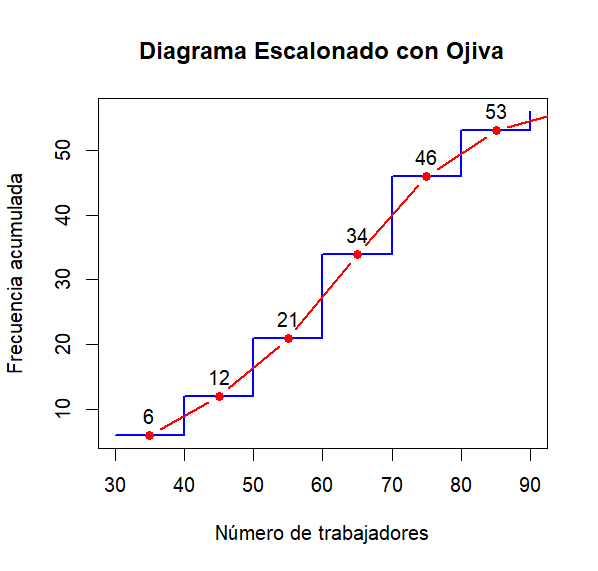
\includegraphics[width=0.8\textwidth]{Diagrama escalonado.png}  % Ajusta el tamaño de la imagen
    \caption{Diagrama escalonado}  % Título de la imagen
    \label{fig:ejemplo1}  % Etiqueta para referenciar la imagen
\end{figure}

\textbf{d) Calcular la media aritmética ($\bar{x}$) y la mediana (Me) para datos agrupados y no agrupados.} (2 puntos)

\begin{lstlisting}[caption=Mostra resultados]
# Media aritmetica agrupada
print(results$grouped_statistics$media)
# Media aritmetica no agrupada
print(results$ungrouped_statistics$media)

# Mediana agrupada
print(results$grouped_statistics$mediana)
# Mediana no agrupada
print(results$ungrouped_statistics$mediana)
\end{lstlisting}

\begin{lstlisting}[caption=Resultados en consola]
> # Media aritmetica agrupada
> print(results$grouped_statistics$media)
[1] 64.28571
> # Media aritmetica no agrupada
> print(results$ungrouped_statistics$media)
[1] 64.16071
>
> # Mediana agrupada
> print(results$grouped_statistics$mediana)
[1] 65.38462
> # Mediana no agrupada
> print(results$ungrouped_statistics$mediana)
[1] 64.5
\end{lstlisting}

\textbf{e) Calcular la moda (Mo) para datos agrupados y no agrupados.} (2 puntos)

\begin{lstlisting}[caption=Mostra resultados]
# Moda agrupada
print(results$grouped_statistics$moda)
# Moda no agrupada
print(results$ungrouped_statistics$moda)
\end{lstlisting}

\begin{lstlisting}[caption=Resultados en consola]
> # Moda agrupada
> print(results$grouped_statistics$moda)
[1] 68
> # Moda no agrupada
> print(results$ungrouped_statistics$moda)
[1] 75
\end{lstlisting}
\end{document}